\section{Макроекономічні моделі на часових шкалах}
\subsection{Класична модель Барро-Гордона}
\label{sec:domain}

\paragraph{} Класична модель Барро-Гордона розглядає уряд (в особі деякого одного політика), яке приймає рішення про заходи впливу на економіку ґрунтуючись на двох факторах. Перший фактор являє собою сумарну функцію добробуту виду

\begin{equation}
 \label{eq:sec:domain:main}
W=\sum_{t=0}^{\infty}\beta^t w_t = \sum_{t=0}^{\infty}\beta^t\left(y_t-\frac{\lambda\pi^2}{2}\right), \quad 0<\beta<1,
\end{equation}
де $\beta^t$ - значимість $t$-ого періоду для добробуту політика, $w_t$ - функція добробуту політика в $t$-ом періодi. При цьому взаємозв'язок між інфляцією та безробіттям задається кривою Лукаса\\
\begin{equation}
	\label{eq:sec:domain:main1}
	y=y^*+\alpha(\pi-\pi^\beta).
\end{equation}

Другий фактор прийняття рішення - це оцінка громадськістю дій уряду у вигляді підтримки або недовіри. Така оцінка в моделі задається через інфляційні очікування, які формуються в період $ t $ наступним чином:
\begin{equation}
\label{eq:sec:domain:main2}
\pi_t = \left\{  \begin{array}{l l}
{\pi}, & \forall t:\pi_t=\tilde{\pi_t}, \\ 
\frac{\alpha}{\lambda}, & \exists s < t : \pi_s \ne \tilde{\pi_s},
\end{array} \right. 
\end{equation}
де $\tilde{\pi}$ - рівень інфляції, який політик обіцяє досягти в результаті впливу на економіку.
\\

Як випливає з~(\ref{eq:sec:domain:main2}), якщо політик поводиться чесно, то громадськість йому довіряє і чекає обіцяний їм рівень інфляції. Якщо політик хоча б раз, обдуривши очікування, провів не ту політику, яку обіцяв, то громадськість йому не вірить. У такому випадку вона очікує відмінний від обіцяного рівень інфляції, який складає	 $\frac{\alpha}{\lambda}$ ,оскільки вважає, що в разі обману політик буде прагнути до того, щоб в економіці встановився саме цей рівень інфляції.
\\

Дійсно, в разі обману політик вибере такий рівень інфляції, який буде максимізувати його функцію добробуту в цьому періоді (припустимо, в періоді $ s $). Оскільки, згідно \eqref{eq:sec:domain:main}-\eqref{eq:sec:domain:main2}, функція добробуту періоду $s$ при $\pi_s\ne\tilde{\pi}$ має вигляд

\begin{equation}
	\label{eq:sec:domain:main3}
	w_s=y^*\alpha\left(\pi_s - \frac{\lambda\pi^2_s}{2} \right),
\end{equation}
то максимізуючий її рівень інфляції буде дорівнювати величині $\frac{\alpha}{\lambda}$, що випливає з першого умови максимізації.\\

Так як репутація політика впливає на інфляційні очікування громадськості, то, згідно з  \eqref{eq:sec:domain:main}-\eqref{eq:sec:domain:main1}, репутація впливає також і на його загальну функцію добробуту. Припустимо, що політик поводиться чесно, тобто проводить ту політику, яку обіцяв. Тоді його загальна функція добробуту приймає вигляд

\begin{equation}
	w^{fair} = \frac{1}{(1-\beta)} \left( y^*-\frac{\lambda\pi^2}{2} \right),
\end{equation}
оскільки в цьому випадку, згідно \eqref{eq:sec:domain:main}-\eqref{eq:sec:domain:main2}, функція добробуту для будь-якого періоду $t$ має вигляд

\begin{equation}
w^{fair}_t = y^*-\frac{\lambda\pi^2}{2}.
\end{equation}

Якщо політик вирішить обдурити очікування громадськості в якийсь (припустимо в нульовий) період часу, то в цьому випадку, згідно  \eqref{eq:sec:domain:main}-\eqref{eq:sec:domain:main2},його функція добробуту в нульовий період буде становити

\begin{equation}
w^{deception}_0 = y^*-\frac{\alpha^2}{2\lambda}-\alpha\tilde{\pi},
\end{equation}
а в усі наступні періоди внаслідок недовіри населення громадськості
\begin{equation}
w^{deception}_0 = y^*-\frac{\alpha^2}{2\lambda}.
\end{equation}

Отже, загальна функція добробуту політика в разі порушення даних обіцянок має вигляд
\begin{equation}
W^{deception} = \frac{1}{(1-\beta)}y^*+\frac{(1-2\beta)\alpha^2}{(1-\beta)2\lambda}-\alpha\tilde{\pi},
\end{equation}

Очевидно, що політику має сенс вести себе чесно тільки за умови $W^{fair} > W^{deception}$ , в іншому випадку він виграє більше від невиконання даних раніше обіцянок.
\\

Виведемо умови, при яких політик поводиться чесно, не обманюючи очікування населення. Скористаємося для цього графічною інтерпретацією цієї проблеми: побудуємо графіки виграшу і програшу політика в разі обману і знайдемо області, в яких виграш буде більше програшу і навпаки.

\begin{figure}[h]
	
	\begin{subfigure}{0.5\textwidth}
		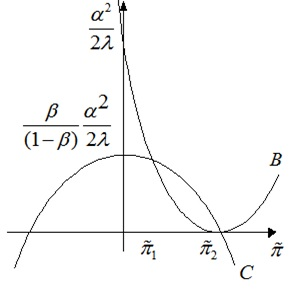
\includegraphics[width=0.9\linewidth]{pic1.jpg} 
		\caption{$\beta < \frac{1}{2}$}
		\label{fig:pic1}
	\end{subfigure}
	\begin{subfigure}{0.5\textwidth}
		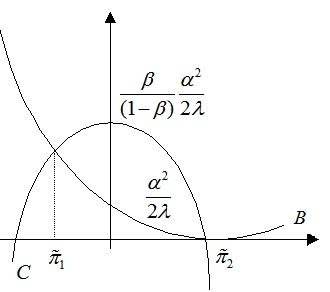
\includegraphics[width=0.9\linewidth]{pic2.jpg}
		\caption{$\beta > \frac{1}{2}$}
		\label{fig:pic2}
	\end{subfigure}
	
	\caption{Графіки втрат і виграшу}
	\label{fig:image2}
\end{figure}

Якщо політик обманює очікування громадськості в нульовий момент часу, то виграш він отримує за рахунок того, що в нульовий момент часу не виправдав сподівань громадськості, а програш - що в подальшому громадськість перестає йому довіряти і завжди чекає більший рівень інфляції, ніж було оголошено.
\\

Отже, виграш обманюючого населення в нульовий момент часу політика
\begin{equation}
B=w^{deception}_0 - w^{fair}_0 = \frac{\lambda\pi^2}{2}+\frac{\alpha^2}{2\lambda}-\alpha\tilde{\pi}
\end{equation}
є квадратичною функцією від декларованого рівня інфляції. Ця функція досягає мінімуму $ B = 0 $ в точці $\tilde{\pi}=\frac{\alpha}{\lambda}$. При $\tilde{\pi}=0$  виграш дорівнює $\frac{\alpha^2}{\lambda}$.

Програш обманюючого населення в нульовий момент часу політика також є квадратичною функцією від декларованого рівня інфляції, оскільки

\begin{equation}
	\label{eq:sec:domain:main4}
C=\sum_{t=1}^{\infty} \beta^t(w^{deception}_t - w^{fair}_t) = -\frac{\lambda\tilde{\pi}^2}{2}+\frac{\alpha^2}{2\lambda}.
\end{equation}



Функція, що задається рівнянням \eqref{eq:sec:domain:main4}, описує параболу,
яка досягає максимуму $C=\frac{\beta}{(1-\beta)}\frac{\alpha^2}{2\lambda} $  в
точцi   $\tilde{\pi}=0$. Значення функції $C$ дорівнює нулю, коли рівень
інфляції становить $\tilde{\pi}\pm\frac{\alpha}{\lambda}$.


Взаєморозміщення графіків втрат і виграшу обманюючого громадськість в нульовий момент часу політика залежить від того, більше чи менше одиниці величина $\frac{\beta}{1-\beta}$.

Якщо   $\frac{\beta}{1-\beta}<1$, то есть  $\beta<\frac{1}{2}$, то функція втрат і функція виграшу перетинаються в точках  $\tilde{\pi}_1>0$ и $\tilde{\pi}_2>0$ \eqref{fig:pic1}, причому  $\tilde{\pi}_1~=~\frac{\alpha(1-2\beta)}{\lambda}$, $\tilde{\pi}_2~=~\frac{\alpha}{\lambda}$. \\
Якщо  $\frac{\beta}{1-\beta}>1,$  тобто  $\beta>\frac{1}{2},$  то функція втрат і функція виграшу перетинаються в точках $\tilde{\pi}_1<0$, $\tilde{\pi}_2>0$ ~(\ref{fig:pic2}).

Таким чином, з проведеного аналізу випливає, що поведінка політика (буде він виконувати обіцянки чи ні) залежить від його відношення до репутації. Якщо для нього репутація не важлива, майбутнє мало впливає на його функцію добробуту $\beta<\frac{1}{2}$, то політику не вигідно вести себе чесно. Оскільки, як видно з \eqref{fig:pic1}, існує досить невисокий рівень інфляції $\tilde{\pi}\in\left(0;\frac{\alpha(1-2\beta)}{\lambda} \right)$ , обіцяючи який він може виграти більше в результаті обману (в порівнянні з чесним поведінкою). Якщо для політика його репутація важлива, майбутнє значимо для його добробуту $\beta<\frac{1}{2}$, то йому має сенс вести себе чесно. Оскільки, як видно з \eqref{fig:pic2}, не існує рівня інфляції близького до нуля, обіцяючи який він може отримати більшу реалізацію своїх цілей в результаті обману в порівнянні з чесною поведінкою.
